\documentclass[11pt]{beamer}
\usepackage{verbatim}
\usepackage{amsmath}
\usepackage{amsthm}
\usepackage{graphics}
\usepackage{color}
\usepackage{stmaryrd}

\title{On Multiphase-Linear Ranking Functions}
\date{\today}
\author{Xie Li}

\begin{document}
\maketitle

\begin{frame}\frametitle{Contributions}
\begin{itemize}
\item Equivalence of different classes of ranking function.

\item Algorithms for converting between ranking functions.

\item Complete solution for ranking functions on integer.

\item Depth bound and iteration bound for M$\Phi$RF.

\end{itemize}
\end{frame}

\begin{frame}\frametitle{Single Path Linear Constraint Loop}
\begin{example}
\begin{center}

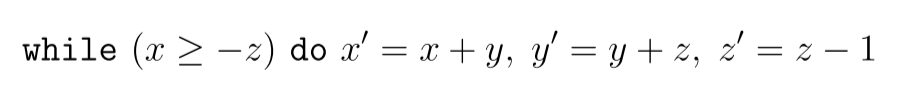
\includegraphics[scale = 0.4]{loopExample.png}

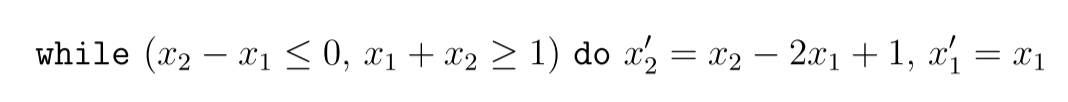
\includegraphics[scale = 0.4]{loopExample1.png}
\end{center}

\end{example}

\begin{definition}[SLC]
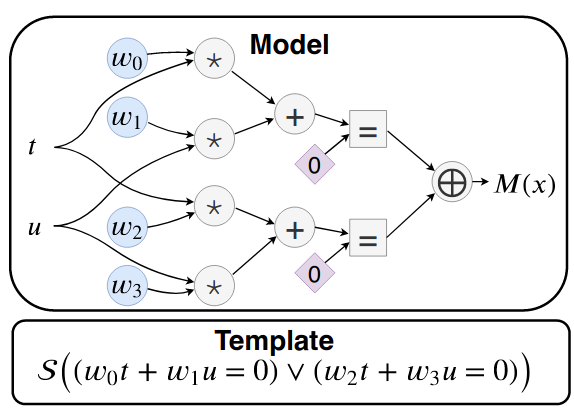
\includegraphics[scale = 0.4]{1.png}


\end{definition}
\begin{center}
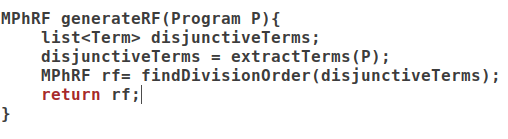
\includegraphics[scale = 0.35]{2.png}

$A''\textbf{x}'' \le \textbf{c}''$
\end{center}


\end{frame}

\begin{frame}\frametitle{Ranking Functions}

\begin{definition}[Linear Ranking Function(LRF)]

$f(x_1, \ldots, x_n) = a_1x_1 + \ldots a_nx_n + a_0$, such that

\begin{itemize}
\item $f(\textbf{x}) \ge 0$ for any $\textbf{x}$ satisfies the loop constraints.

\item $f(\textbf{x}) - f(\textbf{x}') \ge 1$ for any transition from $\textbf{x}$ to $\textbf{x}'$.



\end{itemize}
\end{definition}

\begin{example}
\[\texttt{while }( x - 1 > 0) \texttt{do } x' = x - 1\]

Its LRF: $f(x) = x - 1$
\end{example}

\end{frame}


\begin{frame}\frametitle{Example: Multiphase Ranking Function}
Problem: LRF is not strong enough for all loops.
\begin{example}
\[\texttt{while }( x > -z) \texttt{do } x' = x + y, y' = y + z, z = z - 1\]

$f(x, y, z) = a_1x + a_2y + a_3z + b$

$y$ cannot be used for non-existence of its lower bound.

$f(x, y, z) = x + z$

Problem?
\end{example}

\end{frame}


\begin{frame}\frametitle{Example: Multiphase Ranking Function}
\[\texttt{while }( x > -z) \texttt{do } x' = x + y, y' = y + z, z = z - 1\]

Attempt to use a ranking function that has several phases: 
$\langle z + 1, y + 1, x\rangle$
\begin{center}
\begin{tabular}{|c|c|c|c|c|c|}
\hline 
$x$&$y$&$z$&$z+1$&$y+1$&$x$\\
\hline
$1$&$1$&$1$&$2$&$2$&$1$\\
$2$&$2$&$0$&$1$&$3$&$2$\\
$4$&$2$&$-1$&$0$&$3$&$4$\\
\hline
$6$&$1$&$-2$&$-1$&$2$&$6$\\
$7$&$-1$&$-3$&$-2$&$0$&$7$\\
\hline
$6$&$-4$&$-4$&$-3$&$-3$&$6$\\
$2$&$-8$&$-5$&$-4$&$-7$&$2$\\
\hline
$-6$&$-13$&$-6$&$-5$&$-12$&$-6$\\
\hline
\end{tabular}
\end{center}
\end{frame}



\begin{frame}{Multiphase Ranking Function}
\begin{definition}
Given a set of transitions $T\subseteq \mathbb{Q}^{2n}$, we say $\langle f_1, \ldots, f_d\rangle$ is a multiphase ranking function for $T$ if for every $\textbf{x}'' \in T$, there is an index $i\in [1, d]$, s.t.

\begin{center}
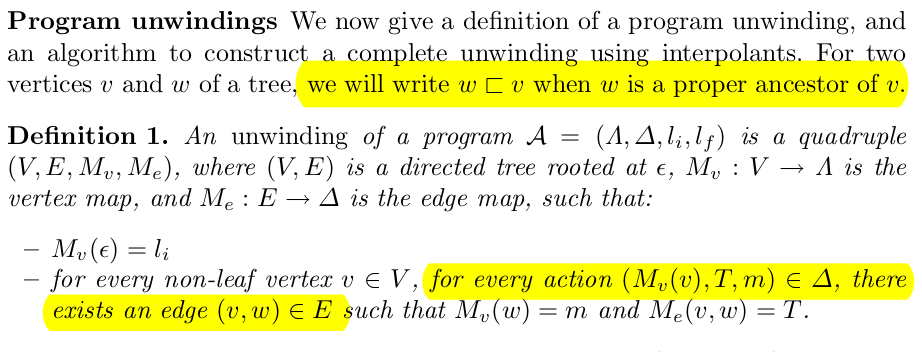
\includegraphics[scale = 0.3]{3.png}
\end{center}
We say that $\textbf{x}''$ is ranked by $f_i$(for the minimal).
\end{definition}


\end{frame}


\begin{frame}\frametitle{Example Revisit}
\[\texttt{while }( x > -z) \texttt{do } x' = x + y, y' = y + z, z = z - 1\]

\begin{center}
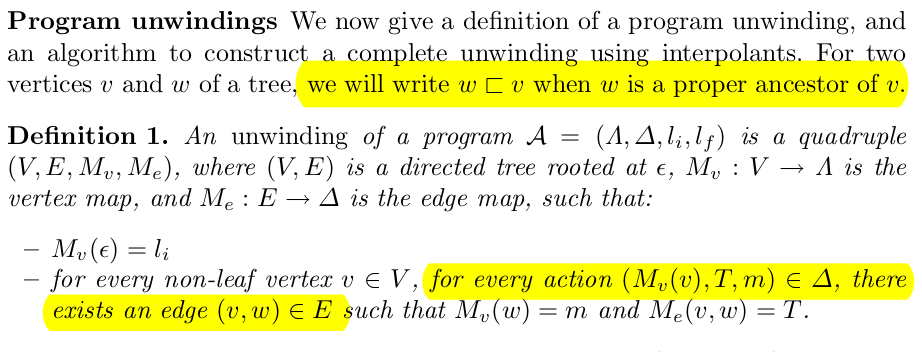
\includegraphics[scale = 0.2]{3.png}

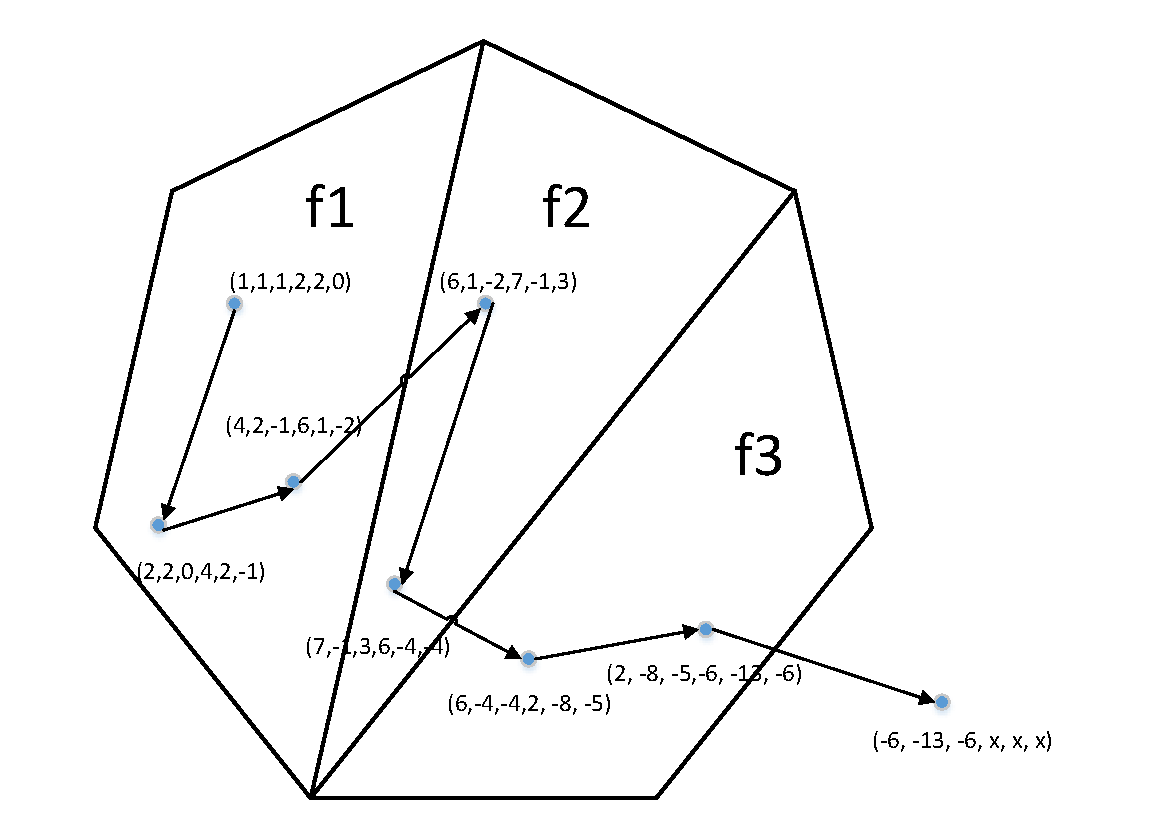
\includegraphics[scale = 0.4]{3.pdf}
\end{center}
\end{frame}


\begin{frame}\frametitle{Nested Ranking Function}
\[\texttt{while }( x > -z) \texttt{do } x' = x + y, y' = y + z, z = z - 1\]

Loop condition: $x + z > 0$. We only want to use this constraint for the ranking function.

$\langle z + 1, y + 1, x + z\rangle$


\begin{definition}[Nested Ranking Function]

A tuple $\langle f_1, \ldots, f_d\rangle$ is a nested ranking function for $T$ if the following requirements are satisfied for all $\textbf{x}''\in T$
\begin{center}
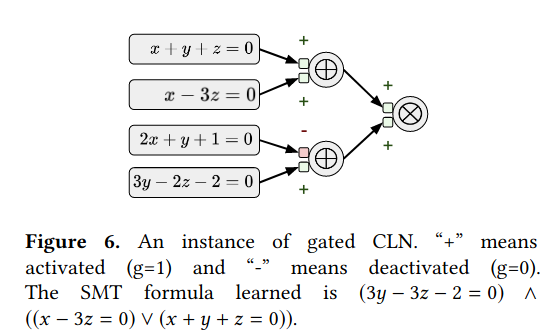
\includegraphics[scale = 0.3]{6.png}

\end{center}

\end{definition}

Let $f_0 = 0$.
\end{frame}

\begin{frame}\frametitle{}



\end{frame}
\end{document}